\documentclass[10pt]{beamer}\usepackage[]{graphicx}\usepackage[]{color}
%% maxwidth is the original width if it is less than linewidth
%% otherwise use linewidth (to make sure the graphics do not exceed the margin)
\makeatletter
\def\maxwidth{ %
  \ifdim\Gin@nat@width>\linewidth
    \linewidth
  \else
    \Gin@nat@width
  \fi
}
\makeatother

\definecolor{fgcolor}{rgb}{0.345, 0.345, 0.345}
\newcommand{\hlnum}[1]{\textcolor[rgb]{0.686,0.059,0.569}{#1}}%
\newcommand{\hlstr}[1]{\textcolor[rgb]{0.192,0.494,0.8}{#1}}%
\newcommand{\hlcom}[1]{\textcolor[rgb]{0.678,0.584,0.686}{\textit{#1}}}%
\newcommand{\hlopt}[1]{\textcolor[rgb]{0,0,0}{#1}}%
\newcommand{\hlstd}[1]{\textcolor[rgb]{0.345,0.345,0.345}{#1}}%
\newcommand{\hlkwa}[1]{\textcolor[rgb]{0.161,0.373,0.58}{\textbf{#1}}}%
\newcommand{\hlkwb}[1]{\textcolor[rgb]{0.69,0.353,0.396}{#1}}%
\newcommand{\hlkwc}[1]{\textcolor[rgb]{0.333,0.667,0.333}{#1}}%
\newcommand{\hlkwd}[1]{\textcolor[rgb]{0.737,0.353,0.396}{\textbf{#1}}}%

\usepackage{framed}
\makeatletter
\newenvironment{kframe}{%
 \def\at@end@of@kframe{}%
 \ifinner\ifhmode%
  \def\at@end@of@kframe{\end{minipage}}%
  \begin{minipage}{\columnwidth}%
 \fi\fi%
 \def\FrameCommand##1{\hskip\@totalleftmargin \hskip-\fboxsep
 \colorbox{shadecolor}{##1}\hskip-\fboxsep
     % There is no \\@totalrightmargin, so:
     \hskip-\linewidth \hskip-\@totalleftmargin \hskip\columnwidth}%
 \MakeFramed {\advance\hsize-\width
   \@totalleftmargin\z@ \linewidth\hsize
   \@setminipage}}%
 {\par\unskip\endMakeFramed%
 \at@end@of@kframe}
\makeatother

\definecolor{shadecolor}{rgb}{.97, .97, .97}
\definecolor{messagecolor}{rgb}{0, 0, 0}
\definecolor{warningcolor}{rgb}{1, 0, 1}
\definecolor{errorcolor}{rgb}{1, 0, 0}
\newenvironment{knitrout}{}{} % an empty environment to be redefined in TeX

\usepackage{alltt}
\usepackage[utf8]{inputenc}
\usepackage{graphicx}
	\usetheme{Warsaw}	
	
	\usepackage{listings}
	\usepackage{color}
	
	\definecolor{dkgreen}{rgb}{0,0.6,0}
	\definecolor{gray}{rgb}{0.5,0.5,0.5}
	\definecolor{mauve}{rgb}{0.58,0,0.82}
	
	\lstset{frame=tb,
		language=R,
		aboveskip=3mm,
		belowskip=3mm,
		showstringspaces=false,
		columns=flexible,
		numbers=none,
		keywordstyle=\color{blue},
		numberstyle=\tiny\color{gray},
		commentstyle=\color{dkgreen},
		stringstyle=\color{mauve},
		breaklines=true,
		breakatwhitespace=true,
		tabsize=3
	}
\IfFileExists{upquote.sty}{\usepackage{upquote}}{}
\begin{document}


\title[Referencias Cruzadas]{Informe de lectura: Dynamic Documents with R and knitr : Cross Reference}
		%Logo Gráfica Escudo Universidad Vectorizado.
		\logo{
\includegraphics[scale=0.08]{escudoud}}
		%Autor, Universidad, Fecha..
		\author{Wilson Ricardo López Sánchez }
		\institute[UD]{Universidad Distrital Francisco Jóse de Caldas}
		\date{\today}


\begin{frame}
	       	%Titulo de la pagina
			\titlepage 
\end{frame}


		
\begin{frame}[fragile]
\frametitle{Código R en latex}
    Para ejecutar código R en un documento. Rnw es necesario utilizar la sintaxis:\\
	\begin{lstlisting}
<<>> =
codigo R
@
	\end{lstlisting}

Para mayor facilidad podemos usar la combinación de teclas \textit{control+alt+i} para generar la sintaxis anterior. \\
\end{frame}

\begin{frame}[fragile]
\frametitle{Ejemplo}
Después de instalar el paquete qqplot2 podemos cargar la librería y el siguiente ejemplo:\\
	\begin{lstlisting}
	<<>> =
	library('ggplot2')
	qplot(carat, price, data = diamonds, color = cut)
	@
	\end{lstlisting}

\end{frame}

\begin{frame}[fragile]
	\frametitle{Gráfica}
    \centering
\begin{knitrout}
\definecolor{shadecolor}{rgb}{0.969, 0.969, 0.969}\color{fgcolor}\begin{kframe}
\begin{alltt}
\hlkwd{library}\hlstd{(}\hlstr{'ggplot2'}\hlstd{)}
\end{alltt}


{\ttfamily\noindent\color{warningcolor}{\#\# Warning: package 'ggplot2' was built under R version 3.2.5}}\begin{alltt}
\hlkwd{qplot}\hlstd{(carat, price,} \hlkwc{data} \hlstd{= diamonds,} \hlkwc{color} \hlstd{= cut)}
\end{alltt}
\end{kframe}
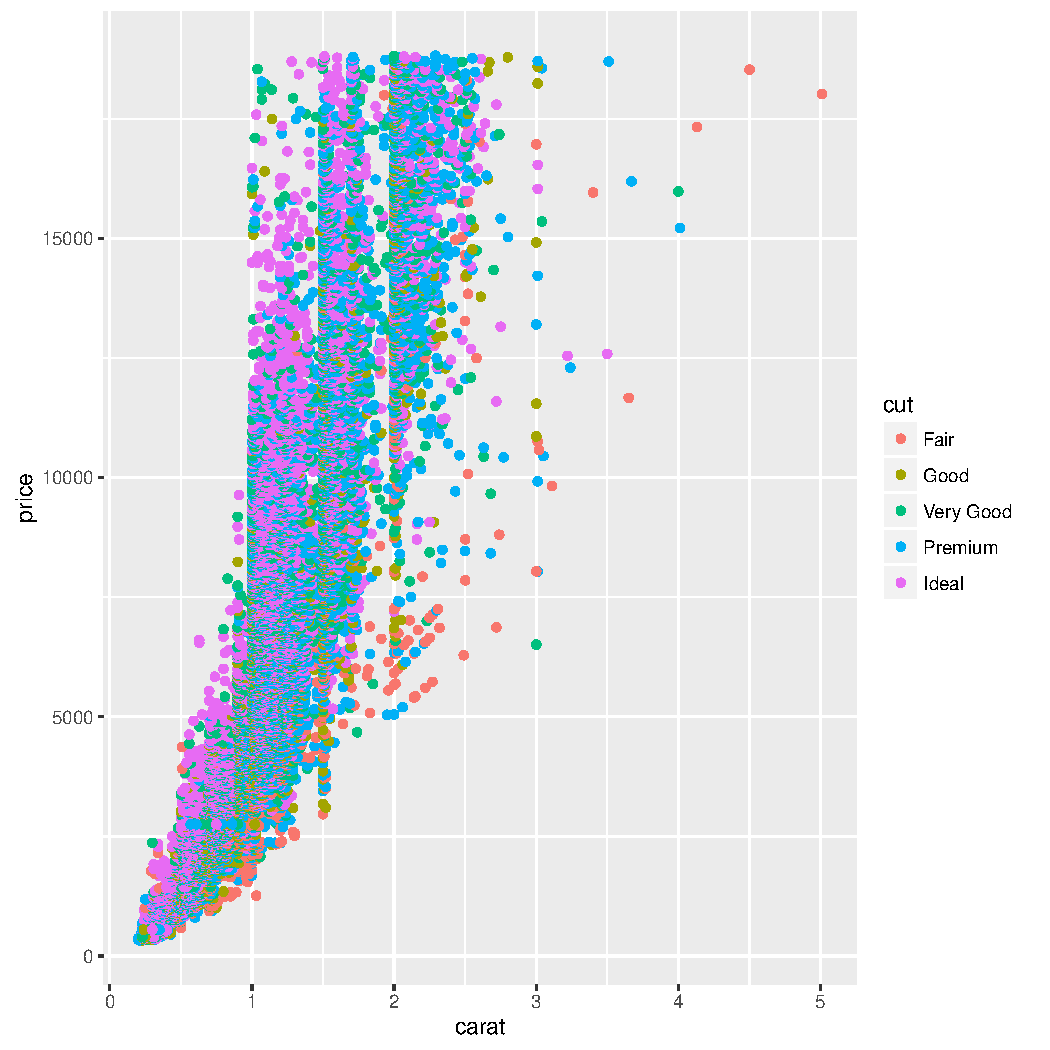
\includegraphics[width=2in]{figure/unnamed-chunk-1-1} 

\end{knitrout}
	\end{lstlisting}
	
\end{frame}




\begin{frame}[fragile]
\frametitle{Ejemplo en Gráficas tema}
	\begin{lstlisting}
	<<temagraficas1, eval=FALSE>> =
	theme(legend.text = element_text(size = 12, angle = 45)) +
	theme(legend.position = "bottom")
	@
	\end{lstlisting}


Ahora podemos realizar nuestra gráfica de la siguiente manera:\\
	\begin{lstlisting}
	<<>> =
	qplot(carat, price, data = diamonds, color = cut) +
	<<temagraficas1>>
	@
	\end{lstlisting}

\end{frame}

\begin{frame}[fragile]
\frametitle{Referencias por segmentos embebidas}
	\begin{lstlisting}
	<<A>> =
	x <- runif(1,0,10)
	@
	<<B>> =
	x
	<<A>>
	x
	@
	\end{lstlisting}
Con lo que obtenemos:
\begin{knitrout}
\definecolor{shadecolor}{rgb}{0.969, 0.969, 0.969}\color{fgcolor}\begin{kframe}
\begin{alltt}
\hlstd{x} \hlkwb{<-} \hlkwd{runif}\hlstd{(}\hlnum{1}\hlstd{,}\hlnum{0}\hlstd{,}\hlnum{10}\hlstd{)}
\end{alltt}
\end{kframe}
\end{knitrout}
\begin{knitrout}
\definecolor{shadecolor}{rgb}{0.969, 0.969, 0.969}\color{fgcolor}\begin{kframe}
\begin{alltt}
\hlstd{x} \hlkwb{<-} \hlkwd{runif}\hlstd{(}\hlnum{1}\hlstd{,}\hlnum{0}\hlstd{,}\hlnum{10}\hlstd{)}
\end{alltt}
\end{kframe}
\end{knitrout}
\end{frame}



\begin{frame}[fragile]
\frametitle{Re-utilización de todo un segmento de código}
	\begin{lstlisting}
<<chunkA, eval=FALSE>> =
x <- 5*6
@
<<chunkA, eval=TRUE>> =
@
	\end{lstlisting}
Lo que da como resultado:\\
\begin{knitrout}
\definecolor{shadecolor}{rgb}{0.969, 0.969, 0.969}\color{fgcolor}\begin{kframe}
\begin{alltt}
\hlstd{x} \hlkwb{<-} \hlnum{5}\hlopt{*}\hlnum{6}
\end{alltt}
\end{kframe}
\end{knitrout}
\begin{knitrout}
\definecolor{shadecolor}{rgb}{0.969, 0.969, 0.969}\color{fgcolor}\begin{kframe}
\begin{alltt}
\hlstd{x} \hlkwb{<-} \hlnum{5}\hlopt{*}\hlnum{6}
\end{alltt}
\end{kframe}
\end{knitrout}
\end{frame}

\begin{frame}[fragile]
\frametitle{Re-utilización de todo un segmento de código}
	\begin{lstlisting}
<<A1>> =
x <- rnorm(1) @
código B1
<<B1>> =
y <- x + 2  @
<<C, ref.label=c('A1', 'B1')>> =  @
	\end{lstlisting}

Lo que da como resultado:código A1
\begin{knitrout}
\definecolor{shadecolor}{rgb}{0.969, 0.969, 0.969}\color{fgcolor}\begin{kframe}
\begin{alltt}
\hlstd{x} \hlkwb{<-} \hlkwd{rnorm}\hlstd{(}\hlnum{1}\hlstd{)}
\end{alltt}
\end{kframe}
\end{knitrout}
Código B1
\begin{knitrout}
\definecolor{shadecolor}{rgb}{0.969, 0.969, 0.969}\color{fgcolor}\begin{kframe}
\begin{alltt}
\hlstd{y} \hlkwb{<-} \hlstd{x} \hlopt{+} \hlnum{2}
\end{alltt}
\end{kframe}
\end{knitrout}
Código C
\begin{knitrout}
\definecolor{shadecolor}{rgb}{0.969, 0.969, 0.969}\color{fgcolor}\begin{kframe}
\begin{alltt}
\hlstd{x} \hlkwb{<-} \hlkwd{rnorm}\hlstd{(}\hlnum{1}\hlstd{)}
\hlstd{y} \hlkwb{<-} \hlstd{x} \hlopt{+} \hlnum{2}
\end{alltt}
\end{kframe}
\end{knitrout}

\end{frame}


\begin{frame}[fragile]
\frametitle{Segmentos por etiqueta}
Se toma como ejemplo el siguiente código de R el cual guardaremos con el nombre de ejemplo1.R

	\begin{lstlisting}
 \#\# ---- D ----
 m <- 2
 n <- 5
 m
 n 
	\end{lstlisting}

   Para llamar el código de R en nuestro documento lo primero es ejecutar el script  read\_chunk de la siguiente manera:\\ 
	\begin{lstlisting}
<<>> =
read\_chunk("ejemplo1.R")
@
	\end{lstlisting}
Posteriormente ya podemos llamar el código por medio de su etiqueta
	\begin{lstlisting}
	<<D>> =	
	@
	\end{lstlisting}


\end{frame}


\begin{frame}[fragile]
\frametitle{Segmentos de códigos basados en líneas}
Como ejemplo guardamos los numero del 1 al 12 en un archivo con el nombre ejemplo2.R\\
1 2 3 4 5 6 7 8 9 10 11 12 \\
Vamos a tomar la línea 1-4,5-8 y 11-12 del archivo de R anterior con ellos formaremos los segmentos de código con las etiquetas E, F y G, dicho proceso se realiza de la siguiente manera:\\ 
\begin{lstlisting}
read\_chunk("ejemplo2.R", labels = c("E", "F", "G"), from = c(1,5, 11), to = c(4,8,12))
\end{lstlisting}

Así podemos llamar cualquiera de los tres segmentos de código en cualquier momento:\\ 
\begin{lstlisting}
<<E>> =
@
<<F>> =
@
<<G>> =
@
\end{lstlisting}
\end{frame}


\begin{frame}
\frametitle{entradas de documentos hijos}
Como ejemplo se toma como documento principal este mismo documento llamado referenciascruzadas.Rnw y como documento hijo crearemos un documento llamado cap1.Rnw con el siguiente código: \\ 

$<<H1>> =$\\
$y<-sum(x^2)$\\
$@$\\

Incluimos el documento hijo de la siguiente forma:

$<<H, child='cap1.Rnw'>>=$\\
$@$\\

\end{frame}

\begin{frame}
\frametitle{Modo independiente}
Tomando el documento cap1.Rnw y agregamos el siguiente comando al documento hijo: \\

$<<parent, include=FALSE>>=$\\
$set\_parent("referenciascruzadas.Rnw ")$\\
$@$\\
Con lo cual el nuevo documento hijo nos quedaría de la siguiente forma: \\ 
$<<parent, include=FALSE>>=$\\
$set\_parent("referenciascruzadas.Rnw ")$\\
$@$\\
$<<H1>>=$\\
$y <- sum(x^2)$\\
$@$\\

 Al compilar el documento hijo observamos que compila sin problemas y con las mismas características del documento principal.
  
\end{frame}


\begin{frame}
\frametitle{Bibliografía}
Codigo R en latex\\
Yihui Xie, 2013\\
Dynamic Documents with R and knitr\\
CRC Press 2016. 2 Ed.\\
\end{frame}


\end{document}
